\newpage
\section{Post-Processing Techniques}
\label{sec:post-processing}

To enhance our analysis results and quantify the performance of our methods, we will explore various post-processing techniques. These techniques aim to improve the results and provide a deeper understanding of the data. We will employ methods such as Principal Component Analysis (PCA), classical Multidimensional Scaling (cMDS), and the k-medoids clustering algorithm. Additionally, we will utilize the silhouette score as an evaluation metric to assess the quality of the clustering.


\subsection{Principal Component Cosine Analysis}
\label{subsec:pca-cosine}

Principal Component Analysis (PCA) is a dimensionality reduction technique that extracts the most significant information from a dataset while minimizing noise. It achieves this by transforming the data into principal components using the eigenvalues and eigenvectors of the covariance matrix. The components with the highest variance are selected to efficiently represent the dataset \cite{pearsonLIIILinesPlanes1901, jolliffePrincipalComponentAnalysis2002}.

In practice, PCA converts an \(n \times n\) distance matrix into an \(n \times k\) matrix (\(k < n\)). After this transformation, pairwise distances in the reduced space are computed using the cosine distance. The cosine distance between two row vectors \(\mathbf{v_1}\) and \(\mathbf{v_2}\) is defined by:

\begin{equation}
    d_{\cos}(\mathbf{v_1}, \mathbf{v_2}) = 1 - \frac{\mathbf{v_1} \cdot \mathbf{v_2}}{\|\mathbf{v_1}\| \|\mathbf{v_2}\|},
    \label{eq:cosine-distance}
\end{equation}

This method calculates the cosine distances between all pairs \((v_i, v_j)\) for \(i, j \in \{1, 2, \ldots, n\}\), reconstructing a symmetric distance matrix. By using cosine distance, we emphasize directional similarity, which effectively handles high-dimensional data. This provides a computationally efficient approach to reconstruct the distance matrix, allowing us to discern and analyze the underlying structure in the data, isolating the most influential characteristics that define data relationships.

\begin{figure}
    \begin{subfigure}[b]{0.48\textwidth}
        \centering
        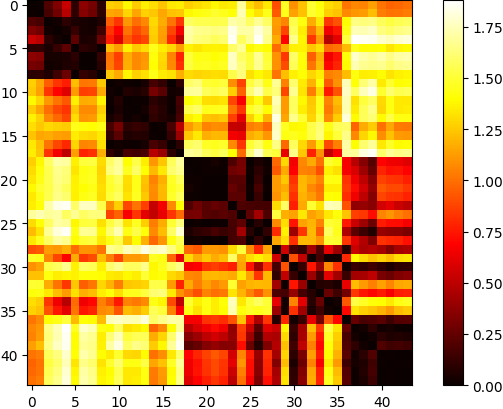
\includegraphics[width=\textwidth]{figures/motion-capture-data/heatmaps/pca_10.png}
        \caption{}
    \end{subfigure}
    \hfill
    \begin{subfigure}[b]{0.48\textwidth}
        \centering
        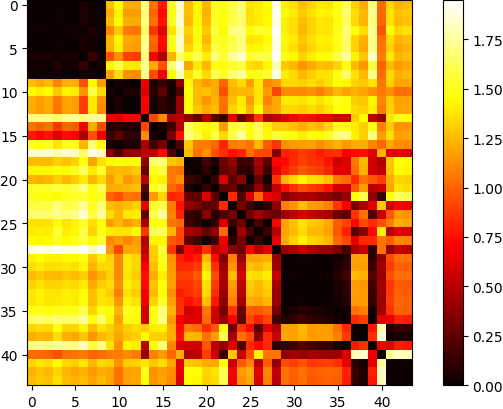
\includegraphics[width=\textwidth]{figures/motion-capture-data/heatmaps/pca_3.png}
        \caption{}
    \end{subfigure}
    \caption[Heat Maps of Cosine Distances after PCA on Reparameterization and Logarithmic Signature Data]{(a) Reparameterization through dynamic programming at a search depth of 10, (b) Logarithmic signature at a truncation level of 3. This figure displays heat maps of the cosine distance matrix following PCA, using data from reparameterization and logarithmic signature as seen in Figure \ref{fig:heatmaps-dynprog} (search depth of 10) and Figure \ref{fig:heatmaps-logsig} (truncation level of 3).}
    \label{fig:heatmap-pca-cosine}
\end{figure}

As shown in both subfigures, the cosine distance matrix after PCA captures the motions as distinct clusters. This indicates that the PCA method effectively reduces the dimensionality of the data, emphasizing the most significant features that define the motion capture data. This also reflects the categorization of the motions, demonstrating PCA's ability to highlight the underlying structure in the data.
\subsection{K-Medoids Clustering}
\label{subsec:kmedoids-clustering}

Given that we are working with a distance matrix, we aim to categorize data using a rigorous method rather than relying solely on visual inspection. K-Medoids clustering, as described in the literature \cite{kaufmannClusteringMeansMedoids1987, schubertFastEagerKMedoids2021}, enables this by partitioning datasets into clusters based on pairwise distances. Given a distance matrix \( D = [d_{ij}]_{i,j=1}^{n} \), k-medoids are selected either randomly or heuristically, here chosen heuristically. Each point is assigned to the nearest medoid, forming clusters \( C_j \). Medoids are updated by selecting the point within each cluster that minimizes the total distance to all other points in the cluster, specifically

\begin{equation}
    m_j = \arg \min_{x \in C_j} \sum_{x_i \in C_j} d(x, x_i).
    \label{eq:k-medoids-update}
\end{equation}

This process iterates until cluster assignments stabilize or changes fall below a threshold. Unlike K-Means, which uses centroids, K-Medoids relies on medoids because means cannot be computed from a distance matrix. The algorithm operates solely on pairwise distances, effectively generalizing K-Means for use with distance matrices.

K-Medoids identifies clusters where points within the same cluster are more similar to each other than to points in different clusters. It retains the advantages of K-Means while being suitable for datasets where only pairwise distances are available, providing a robust and interpretable clustering method for rigorous mathematical analysis.

In Table \ref{tab:k-medoids-motion-capture}, we present the results of K-Medoids clustering on the motion capture data. We applied this method to the distances created by reparameterization by dynamic programming search depth 10 and logarithmic signature with truncation level 3. This was done twice: once on the original distances and once on the reduced distances, where we used PCA combined with cosine similarity to reduce the dimensionality of the data (see Subsection \ref{subsec:pca-cosine}). The values have been mapped to facilitate comparison, as the clusters are not necessarily ordered in the same way, as the number assigned to each cluster is arbitrary.

\begin{longtable}{lrrrr}
    \caption{K-Medoids clustering on motion capture data} \label{tab:k-medoids-motion-capture} \\
    \toprule
    Motion & Reparam & LogSig & Reparam (Red) & LogSig (Red) \\
    \midrule
    \endfirsthead
    
    \toprule
    Motion & Reparam & LogSig & Reparam (Red) & LogSig (Red) \\
    \midrule
    \endhead
    
    \bottomrule
    \endfoot
    
    \bottomrule
    \endlastfoot
    
    Forward Jump & 0 & 0 & 0 & 0 \\
Forward Jump & 0 & 0 & 0 & 0 \\
Forward Jump & 0 & 0 & 0 & 0 \\
Forward Jump & 0 & 0 & 0 & 0 \\
Forward Jump & 0 & 0 & 0 & 0 \\
Forward Jump & 0 & 0 & 0 & 0 \\
Forward Jump & 0 & 0 & 0 & 0 \\
Forward Jump & 0 & 0 & 0 & 0 \\
Forward Jump & 0 & 0 & 0 & 0 \\
Run/Jog & 1 & 1 & 1 & 1 \\
Run/Jog & 1 & 1 & 1 & 1 \\
Run/Jog & 1 & 1 & 1 & 1 \\
Run/Jog & 1 & 1 & 1 & 1 \\
Run/Jog & 4 & 2 & 1 & 2 \\
Run/Jog & 4 & 1 & 1 & 1 \\
Run/Jog & 1 & 1 & 1 & 1 \\
Run/Jog & 1 & 1 & 1 & 1 \\
Run/Jog & 4 & 1 & 1 & 1 \\
Walk & 2 & 2 & 2 & 2 \\
Walk & 2 & 2 & 2 & 2 \\
Walk & 2 & 2 & 2 & 2 \\
Walk & 2 & 2 & 2 & 2 \\
Walk & 2 & 2 & 2 & 2 \\
Walk & 4 & 4 & 2 & 2 \\
Walk & 2 & 2 & 2 & 2 \\
Walk & 2 & 2 & 2 & 2 \\
Walk & 2 & 4 & 2 & 2 \\
Walk & 2 & 2 & 2 & 2 \\
Boxing & 4 & 4 & 3 & 4 \\
Boxing & 3 & 3 & 3 & 3 \\
Boxing & 3 & 3 & 4 & 3 \\
Boxing & 3 & 3 & 3 & 3 \\
Boxing & 3 & 3 & 3 & 3 \\
Boxing & 3 & 3 & 3 & 3 \\
Boxing & 4 & 3 & 3 & 3 \\
Boxing & 4 & 2 & 3 & 3 \\
Boxing & 4 & 0 & 4 & 3 \\
Climb Stairs & 4 & 4 & 4 & 4 \\
Climb Stairs & 4 & 4 & 4 & 4 \\
Climb Stairs & 4 & 3 & 4 & 3 \\
Climb Stairs & 4 & 0 & 4 & 3 \\
Climb Stairs & 4 & 4 & 4 & 4 \\
Climb Stairs & 4 & 4 & 4 & 4 \\
Climb Stairs & 4 & 4 & 4 & 4 \\

\end{longtable}


\subsection{Classical Multidimensional Scaling (cMDS)}
\label{subsec:cMDS}

Classical multidimensional scaling (cMDS) is a technique used to visualize the distances between entities in a lower-dimensional space, typically two or three dimensions. Unlike Principal Component Analysis (PCA), which aims to maximize data variation, cMDS focuses on preserving the original distances between points as accurately as possible. This approach is detailed in Chapter 6 of Wang (2012) \cite{wangClassicalMultidimensionalScaling2012}.
Your section on Classical Multidimensional Scaling (cMDS) is clear and well-structured. Below is a refined version to enhance rigor, flow, and conciseness.

Given a set of \( n \) entities represented by a distance matrix \( D = [d_{ij}]_{i,j=1}^{n} \), cMDS seeks a configuration \( \mathcal{Y} = \{y_1, \ldots, y_n\} \) in \( \mathbb{R}^d \) such that the Euclidean distances \( d_{\mathcal{Y}}(y_i, y_j) \) between points \( y_i \) and \( y_j \) in \( \mathcal{Y} \) approximate the original distances \( d_{ij} \):

\begin{equation}
    d_{\mathcal{Y}} (y_i, y_j) \approx d_{ij}, \quad \forall i, j.
    \label{eq:cmds-approximation}
\end{equation}

First, the distance matrix \( D \) is centered using the centering matrix \( H = I - \frac{1}{n} \mathbf{1} \mathbf{1}^T \), where \( I \) is the identity matrix and \( \mathbf{1} \) is a vector of ones. The centered Gram matrix \( G^C \) is calculated as:

\begin{equation}
    G^C = -\frac{1}{2} H D^2 H,
    \label{eq:cmds-gram-matrix}
\end{equation}
where \( D^2 \) is the element-wise square of the distance matrix \( D \). Next, eigendecomposition is performed on \( G^C \) to obtain its eigenvalues \( \lambda_i \) and corresponding eigenvectors \( u_i \):

\begin{equation}
    G^C = U \Sigma U^T,
    \label{eq:cmds-eigen-decomposition}
\end{equation}
where \( U = [u_1, u_2, \ldots, u_r] \) and \( \Sigma = \text{diag}(\lambda_1, \lambda_2, \ldots, \lambda_r) \). The eigenvalues and eigenvectors are sorted in descending order of the eigenvalues. To construct the configuration matrix \( Y \), the top \( d \) eigenvalues and their corresponding eigenvectors are selected. Let \( U_d = [u_1, u_2, \ldots, u_d] \) and \( \Sigma_d = \text{diag}(\sqrt{\lambda_1}, \sqrt{\lambda_2}, \ldots, \sqrt{\lambda_d}) \). The configuration matrix \( Y \) is then given by:

\begin{equation}
    Y = U_d \Sigma_d.
    \label{eq:cmds-configuration-matrix}
\end{equation}

For visualization, the first two columns of \( Y \) are typically plotted to provide a two-dimensional representation of the data.


%%%%%%%%%%%%%%%%%%%%%%%%%%%%%%%%%%%%%%%%%%%%%%%%%%%%%%%%%%%%

By applying cMDS to the distance matrices generated by the reparameterization search at depth 10 and logarithmic signature truncation at level 3, the motion capture data can be visualized in two dimensions. This visualization is performed for both the original distances and the reduced distances obtained by PCA combined with cosine similarity. The cluster assignments obtained by K-Medoids clustering are included to better understand the data structure. The original reparameterization with clustering is shown in Figure \ref{fig:2d-reparameterization-depth10}, the reduced reparameterization with clustering in Figure \ref{fig:2d-reparameterization-depth10_reduced}, the original logarithmic signature with clustering in Figure \ref{fig:2d-logsig-level3}, and the reduced logarithmic signature with clustering in Figure \ref{fig:2d-logsig-level3_reduced}.

The figures demonstrate that the clustering utilizing the reparameterization method is quite distinct, especially when colored by the true cluster assignments. The reduced data show even clearer cluster formations in the 2D space, with the reduced clustering numbers more aligned with the true cluster assignments.

In the logarithmic signature method, the data are not as distinct as in the reparameterization method, for both the original and reduced data. However, the reduced data still show clearer cluster formations in 2D space.

In the reduced reparameterization data, "forward jump", "run/jog" and "walk" are distinct, while "boxing" and "climbing stairs" are somewhat mixed but still relatively distinct. For the logarithmic signature method, only "forward jump" is clearly separate, while "run/jog", "walk" and "climbing stairs" are somewhat distinct, with "boxing" mixed with the other clusters. This suggests that the "boxing" movement may resemble other movements, making it less distinct.

Overall, these results indicate that distinguishing real motion capture data using these methods is feasible. The application of post-processing techniques such as PCA with cosine distance, cMDS, and clustering enhances the clarity of the results compared to the heatmap figures \ref{fig:heatmaps-dynprog}, \ref{fig:heatmaps-logsig}.

\begin{figure}
    \centering
    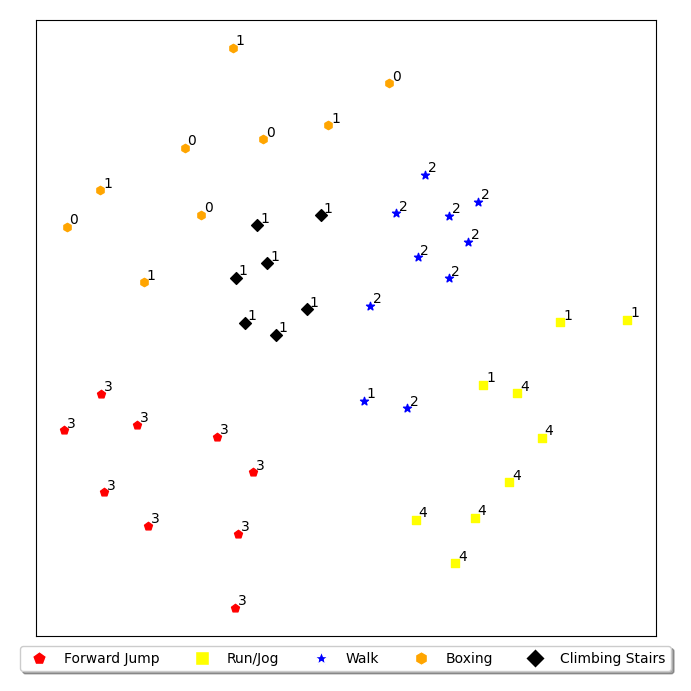
\includegraphics[width=0.99\textwidth]{figures/motion-capture-data/2d_plots/reparameterization_depth10}
    \caption[2D cMDS Visualization of Reparameterized Motion Capture Data (Search Depth 10)]{2D visualization using cMDS of the reparameterization of motion capture data with dynamic programming using search depth 10. Colors and shapes represent the true cluster assignments, while the numbers indicate cluster assignments generated by K-Medoids clustering, with five clusters.}
    \label{fig:2d-reparameterization-depth10}
\end{figure}

\begin{figure}
    \centering
    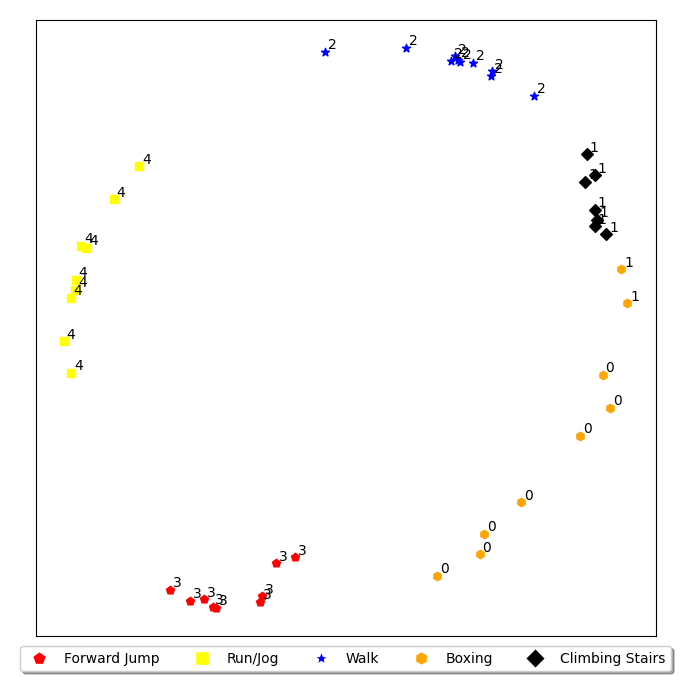
\includegraphics[width=0.99\textwidth]{figures/motion-capture-data/2d_plots/reparameterization_depth10_red}
    \caption[2D cMDS Visualization of PCA-Reduced Reparameterized Motion Capture Data (Search Depth 10)]{2D visualization using cMDS of the reduced reparameterization of motion capture data, reduced to 4 dimensions using PCA and rebuilt with cosine distance, with dynamic programming using search depth 10. Colors and shapes represent the true cluster assignments, while the numbers indicate cluster assignments generated by K-Medoids clustering, with five clusters.}
    \label{fig:2d-reparameterization-depth10_reduced}
\end{figure}

\begin{figure}
    \centering
    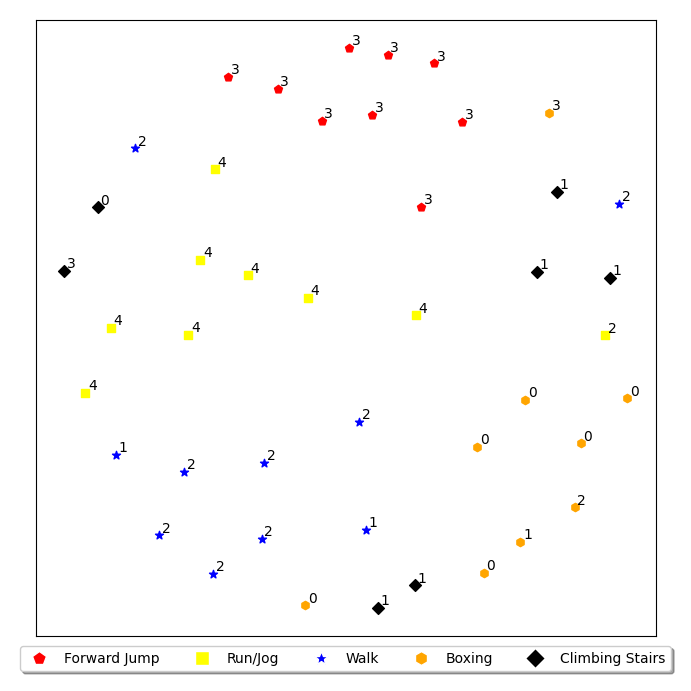
\includegraphics[width=0.99\textwidth]{figures/motion-capture-data/2d_plots/logsig_level3}
    \caption[2D cMDS Visualization of Logarithmic Signature Motion Capture Data (Truncation Level 3)]{2D visualization using cMDS of the logarithmic signature of motion capture data with truncation level 3. Colors and shapes represent the true cluster assignments, while the numbers indicate cluster assignments generated by K-Medoids clustering, with five clusters.}
    \label{fig:2d-logsig-level3}
\end{figure}

\begin{figure}
    \centering
    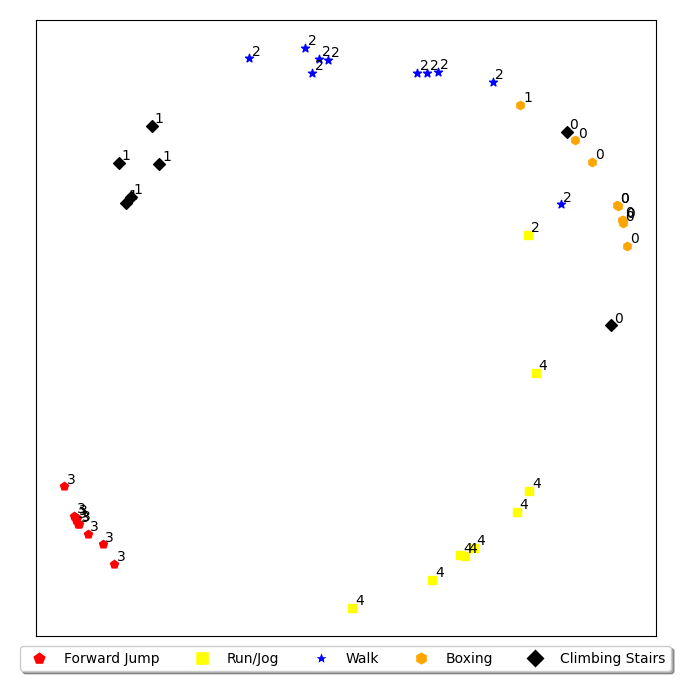
\includegraphics[width=0.99\textwidth]{figures/motion-capture-data/2d_plots/logsig_level3_red}
    \caption[2D cMDS Visualization of PCA-Reduced Logarithmic Signature Motion Capture Data (Truncation Level 3)]{2D visualization using cMDS of the reduced logarithmic signature of motion capture data, reduced to 4 dimensions using PCA and rebuilt with cosine distance, with truncation level 3. Colors and shapes represent the true cluster assignments, while the numbers indicate cluster assignments generated by K-Medoids clustering, with five clusters.}
    \label{fig:2d-logsig-level3_reduced}
\end{figure}


\newpage
\FloatBarrier
\subsection{Silhouette Score}
\label{subsec:silhouette-score}

The Silhouette Score, introduced by Rousseeuw \cite{rousseeuwRousseeuwSilhouettesGraphical1987}, evaluates clustering quality by quantifying how well objects match their own clusters compared to other clusters.

For each point \( i \), let \( a(i) \) be the average distance to all other points in the same cluster, and \( b(i) \) be the average distance to all points in the nearest different cluster. The Silhouette Score for point \( i \) is:

\begin{equation}
    s(i) = \frac{b(i) - a(i)}{\max\{a(i), b(i)\}},
    \label{eq:silhouette-score}
\end{equation}
where \( -1 \leq s(i) \leq 1 \). A high \( s(i) \) indicates that the point is well-matched to its own cluster and poorly matched to other clusters.

The overall Silhouette Score is the mean of the scores for all points, with higher scores indicating better-defined clusters. This metric robustly evaluates clustering performance, ensuring meaningful and interpretable groupings.

\begin{table}[h]
    \centering
    \begin{tabular}{llll}
\toprule
\midrule
Reparam & LogSig & Reparam (Red) & LogSig (Red) \\
0.115690 & 0.072149 & 0.791245 & 0.751394 \\
\bottomrule
\end{tabular}

    \caption{Silhouette Scores for K-Medoids Clustering}
    \label{tab:silhouette-scores}
\end{table}

In Table \ref{tab:silhouette-scores}, we present the Silhouette Scores for K-Medoids clustering on the motion capture data (see Table \ref{tab:k-medoids-motion-capture}). The scores indicate that the reparameterization method has a higher score (0.115) compared to the logarithmic signature method (0.072). Additionally, the scores significantly increase when the dimensionality of the data is reduced, reaching 0.791 and 0.751 when utilizing reparameterization and logarithmic signature, respectively. This suggests that clustering is more well-defined when the data is reduced.
